\documentclass[a4paper,14pt, unknownkeysallowed]{extreport}

\usepackage{cmap} % Улучшенный поиск русских слов в полученном pdf-файле
\usepackage[T2A]{fontenc} % Поддержка русских букв
\usepackage[utf8]{inputenc} % Кодировка utf8
\usepackage[english,russian]{babel} % Языки: русский, английский
\usepackage{enumitem}


\usepackage{threeparttable}

\usepackage[14pt]{extsizes}

\usepackage{caption}
\captionsetup{labelsep=endash}
\captionsetup[figure]{name={Рисунок}}

% \usepackage{ctable}
% \captionsetup[table]{justification=raggedleft,singlelinecheck=off}

\usepackage{amsmath}

\usepackage{geometry}
\geometry{left=30mm}
\geometry{right=15mm}
\geometry{top=20mm}
\geometry{bottom=20mm}

\usepackage{titlesec}
\titleformat{\section}
	{\normalsize\bfseries}
	{\thesection}
	{1em}{}
\titlespacing*{\chapter}{0pt}{-30pt}{8pt}
\titlespacing*{\section}{\parindent}{*4}{*4}
\titlespacing*{\subsection}{\parindent}{*4}{*4}

\usepackage{setspace}
\onehalfspacing % Полуторный интервал

\frenchspacing
\usepackage{indentfirst} % Красная строка
\setlength{\parindent}{1.25cm}

\usepackage{titlesec}
\titleformat{\chapter}{\LARGE\bfseries}{\thechapter}{20pt}{\LARGE\bfseries}
\titleformat{\section}{\Large\bfseries}{\thesection}{20pt}{\Large\bfseries}

\usepackage{multirow}
\usepackage{listings}
\usepackage{xcolor}

% Для листинга кода:
\lstset{ %
language=caml,                 % выбор языка для подсветки (здесь это С)
basicstyle=\small\sffamily, % размер и начертание шрифта для подсветки кода
numbers=left,               % где поставить нумерацию строк (слева\справа)
stepnumber=1,                   % размер шага между двумя номерами строк
numbersep=5pt,                % как далеко отстоят номера строк от подсвечиваемого кода
showspaces=false,            % показывать или нет пробелы специальными отступами
showstringspaces=false,      % показывать или нет пробелы в строках
showtabs=false,             % показывать или нет табуляцию в строках
frame=single,              % рисовать рамку вокруг кода
tabsize=2,                 % размер табуляции по умолчанию равен 2 пробелам
captionpos=t,              % позиция заголовка вверху [t] или внизу [b] 
breaklines=true,           % автоматически переносить строки (да\нет)
breakatwhitespace=false, % переносить строки только если есть пробел
escapeinside={\#*}{*)}   % если нужно добавить комментарии в коде
}



% plot
\usepackage{graphicx}
\usepackage{pgfplots}
\usepackage{filecontents}
\usetikzlibrary{datavisualization}
\usetikzlibrary{datavisualization.formats.functions}

\graphicspath{ {img/} }


\usepackage{subcaption}

\captionsetup{labelsep=endash}
\captionsetup[figure]{name={Рисунок}}



\usepackage[justification=centering]{caption} % Настройка подписей float объектов

\usepackage[unicode,pdftex]{hyperref} % Ссылки в pdf
\hypersetup{hidelinks}

\usepackage{csvsimple}

\newcommand{\code}[1]{\texttt{#1}}

\begin{document}
	
\begin{titlepage}
	\newgeometry{pdftex, left=2cm, right=2cm, top=2.5cm, bottom=2.5cm}
	\fontsize{12pt}{12pt}\selectfont
	\noindent \begin{minipage}{0.15\textwidth}
		
\includegraphics[width=\linewidth]{img/main_logo.jpg}
	\end{minipage}
	\noindent\begin{minipage}{0.9\textwidth}\centering
		\textbf{Министерство науки и высшего образования Российской Федерации}\\
		\textbf{Федеральное государственное бюджетное образовательное учреждение высшего образования}\\
		\textbf{«Московский государственный технический университет имени \newline Н. Э. Баумана}\\
		\textbf{(национальный исследовательский университет)»}\\
		\textbf{(МГТУ им. Н. Э.~Баумана)}
	\end{minipage}
	
	\noindent\rule{18cm}{3pt}
	\newline\newline
	\noindent ФАКУЛЬТЕТ $\underline{\text{«Информатика и системы управления»~~~~~~~~~~~~~~~~~~~~~~~~~~~~~~~~~~~~~~~~~~~~~~~~~~~~~~~}}$ \newline\newline
	\noindent КАФЕДРА $\underline{\text{«Программное обеспечение ЭВМ и информационные технологии»~~~~~~~~~~~~~~~~~~~~~~~}}$\newline\newline\newline\newline\newline\newline\newline
	
	
	\begin{center}
		\noindent\begin{minipage}{1.3\textwidth}\centering
		\Large\textbf{   ~~~ Лабораторная работа №3}\newline
		\textbf{по дисциплине "Анализ Алгоритмов"}\newline\newline\newline
		\end{minipage}
	\end{center}
	
	\noindent\textbf{Тема} 			$\underline{\text{Алгоритмы сортировки}}$\newline\newline
	\noindent\textbf{Студент} 		$\underline{\text{Светличная А.А.}}$\newline\newline
	\noindent\textbf{Группа} 		$\underline{\text{ИУ7-53Б}}$\newline\newline
	\noindent\textbf{Преподаватель} $\underline{\text{Волкова Л. Л., Строганов Ю.В.}}$\newline
	
	\begin{center}
		\vfill
		Москва~---~\the\year
		~г.
	\end{center}
	\restoregeometry
\end{titlepage}
	
	\setcounter{page}{2}
	\tableofcontents
	
\newpage
\chapter*{Введение}
	
\addcontentsline{toc}{chapter}{Введение}
	
\textbf{Сортировка} -- процесс перестановки объектов данного множества в определенном порядке. 
Сортировка служит для последующего облегчения поиска элементов в отсортированном множестве. При этом соритровка является примером огромного разообразия алгоритмов, выполняющих одну и ту же задачу. 
Несмотря на большое количество алгоритмов сортировки, любой из них можно разбить на три основные части:

\begin{itemize}
    \item сравнение, определяющее порядок элементов в паре;
    \item перестановка, меняющая элементы в паре местами;
    \item сам сортирующий алгоритм, который выполняет два предыдущих шага до полного упорядочивания.
\end{itemize}

Ввиду большого количества алгоритмов сортировки одни из них имеют преимущества
над другими, что приводит к необходимости их сравнительного анализа
\cite{intro}.

	
\chapter{Аналитическая часть}
	
\section{Цель и задачи}
	
\textbf{Целью данной работы} является исследование алгоритмов сортировок -- блочной, пирамидальной, бусинами. 

Для этого в ходе исследования алгоритмов требуется решить следующие \textbf{задачи}:

\begin{enumerate}
	\item[1)] изучить и рассмотреть выбранные алгоритмы сортировок;
	\item[2)] построить блок-схемы выбранных алгоритмов;
	\item[3)] реализовать каждый из алгоритмов;
	\item[4)] рассчитать их трудоемкость;
	\item[5)] экспериментально оценить временные характеристики алгоритмов;
	\item[6)] сделать вывод на основании проделанной работы.
\end{enumerate}
	
	
\section{Пирамидальная сортировка}

\textbf{Пирамидальная сортировка} (или сортировка кучей, Heap sort) -- это метод сортировки сравнением, основанный на такой структуре данных как двоичная куча.

\textbf{Двоичная куча} -- это законченное двоичное дерево, в котором элементы хранятся в особом порядке: значение в родительском узле больше (или меньше) значений в его двух дочерних узлах. Первый вариант называется max-heap, а второй — min-heap. Куча может быть представлена двоичным деревом или массивом.

\textbf{Суть пирамидальной сортировки}:

\begin{enumerate}
	\item[1)] построить max-heap из входных данных;
	\item[2)] заменинть самый большой элемент из корня кучи на последний элемент кучи;
	\item[3)] уменьшить размер кучи на 1;
	\item[4)] преобразовать полученное дерево в max-heap с новым корнем;
	\item[5)] повторить вышеуказанные действий, пока размер кучи больше 1.
\end{enumerate}
	
\section{Cортировка бусинами}

\textbf{Cортировка бусинами} (или бисерная сортировка, Bead sort) -- основана на внешнем виде и принципе действия античного «калькулятора».

\textbf{Суть сортировки бусинами} для набора натуральных чисел:

\begin{enumerate}
	\item[1)] выложить друг под другом каждое число в виде горизонтального ряда из соответствующего числа шариков;
	\item[2)] сдвинуть шарики вниз до упора;
	\item[3)] переключиться на горизонтали и пересчитать бусинки в каждом ряду;
	\item[4)] получить упорядоченный набор чисел.
\end{enumerate}

\textbf{Ограничения применимости}: 

\begin{itemize}
    \item для натруальных чисел -- метод работает без дополнительных действий;
    \item для целых чисел -- обрабатывать отрицательные числа отдельно;
    \item для дробных чисел -- привести к целым, умножив на 10k;
    \item для строк -- представить в виде целого положительного числа.
\end{itemize}
	
\section{Блочная сортировка}

\textbf{Блочная сортировка} (или карманная сортировка, корзинная сортировка, Bucket sort) — алгоритм сортировки, в котором сортируемые элементы распределяются между конечным числом отдельных блоков так, чтобы все элементы в каждом следующем по порядку блоке были всегда больше (или меньше), чем в предыдущем. Каждый блок затем сортируется отдельно, либо рекурсивно тем же методом, либо другим. Затем элементы помещаются обратно в массив.
	
\section*{Вывод}
	
В данном разделе были изучены и рассмотрены алгоритмы сортировок по варианту.
	
\chapter{Конструкторская часть}

\section{Описания алгоритмов}
	
На рисунках \ref{fig:heap_sort}, \ref{fig:heap_sort}, \ref{fig:bucket_sort} представлены схемы алгоритмов пирамидальной, бисерной и блочной сортировки соответсвенно.

\begin{figure}[h!]
	\centering
	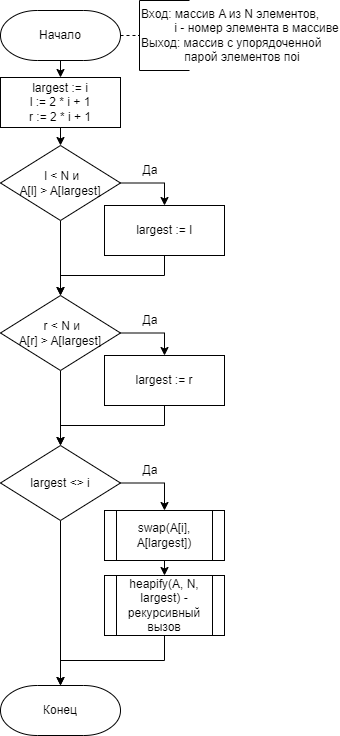
\includegraphics[width=0.52\linewidth]{img/heapify.png}
	\caption{Схема алгоритма рекурсивной  подгромма пирамидальной сортировки}
	\label{fig:heapify}
\end{figure}
	
\begin{figure}[h!]
	\centering
	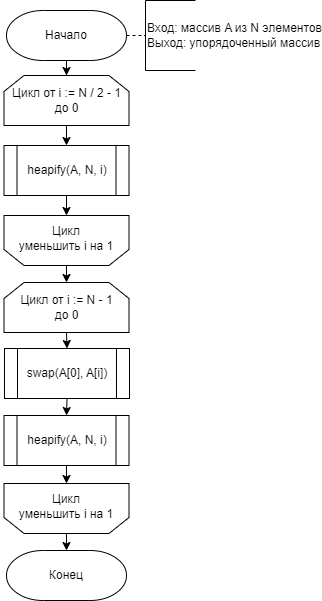
\includegraphics[width=0.7\linewidth]{img/heap_sort.png}
	\caption{Схема алгоритма пирамидальной сортировки}
	\label{fig:heap_sort}
\end{figure}
	
\begin{figure}[h!]
	\centering
	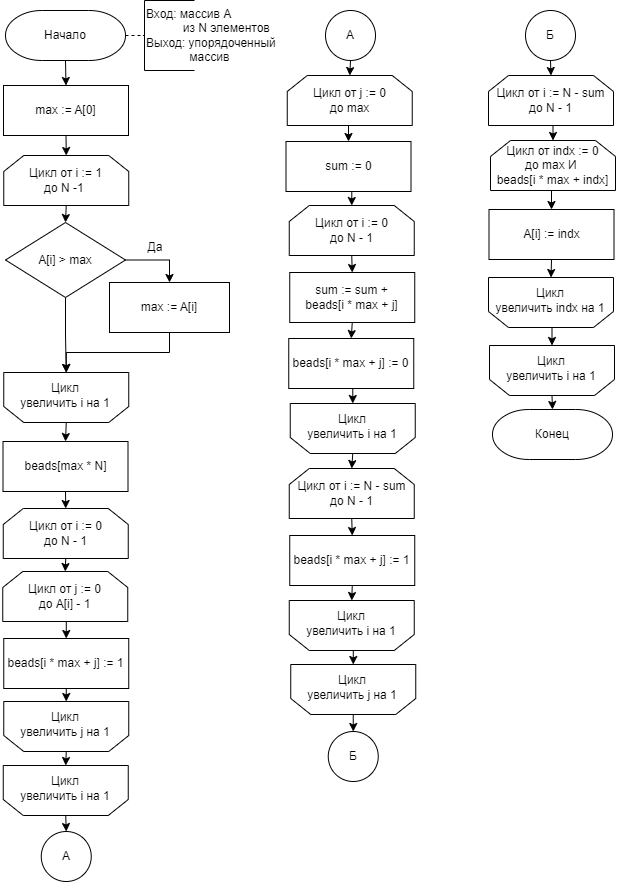
\includegraphics[width=1\linewidth]{img/bead_sort.png}
	\caption{Схема алгоритма бисерной сортировки}
	\label{fig:bead_sort}
\end{figure}
	
\begin{figure}[h!]
	\centering
	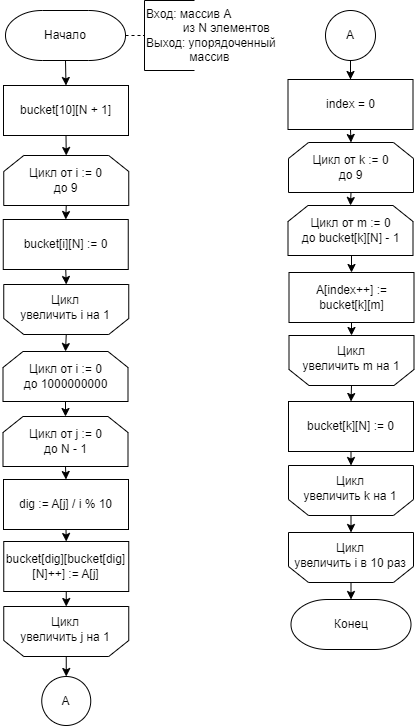
\includegraphics[width=0.8\linewidth]{img/bucket_sort.png}
	\caption{Схема алгоритма блочной сортировки}
	\label{fig:bucket_sort}
\end{figure}

\section{Модель вычислений трудоемкости}

\begin{enumerate}
	\item[1)] Операции, имеющие трудоемкость 1:
	\begin{equation*}
	   +, -, \%, ==, !=, <, >, <=, >=, [], ++, {-}-, {<}<, {>}>.
	\end{equation*}
	\item[2)] Операции, имеющие трудоемкость 2:
	\begin{equation*}
		*, /.
	\end{equation*}
	\item[3)] Трудоемкость оператора выбора if условие then A else B рассчитывается как:
	\begin{equation*}
		f_{if} = f_{\text{условия}} +
	\begin{cases}
		f_A, & \text{условие выполняется,}\\
		f_B, & \text{иначе.}
	\end{cases}
	\end{equation*}
	\item[4)] Трудоемкость вызова функции равна 0.
	\item[5)] Трудоемкость цикла рассчитывается как:
	\begin{equation*}
		f_{for} = f_{\text{инициализации}} + f_{\text{сравнения}} + N(f_{\text{тела}} + f_{\text{инкремента}} + f_{\text{сравнения}}).
	\end{equation*}
\end{enumerate}

\section{Оценка сложности алгоритмов}

\begin{enumerate}
    \item \textbf{Блочная сортировка:} $f = 108N + 630K + 570$,
     где K --- количество блоков. 
     
     Однако сложность сортировки зависит и от сложности сортировки, выбранной для сортировки элементов в блоках.
     Таким образом, для данной сортировки определен только лучший случай --- $O(N)$.
    
    \item \textbf{Пирамидальная сортировка.}
    
    Функция сортировки состоит из двух модулей: процедура просеивания элемента через пирамиду и основная функция сортировки.

    Для начала рассмотрим процедуру просеивания элемента через пирамиду.
    
    Введем $T(N)$ --- трудоемкость процедуры просеивания элемента через пирамиду, состоящую из $N$ элементов. Это время для левой части пирамиды определяется по следующему далее соотношению.
    \begin{equation}
       T(N)=Q(1)+T(\frac{2}{3}N),
    \end{equation}
     где Q(1) – трудоемкость, которая определяется процедурой обмена элемента с одним из своих «потомков».
     
     Для просеивания элемента, расположенного на высоте $h$ требуется $Q(h)$ операций. Число вершин на высоте h меньше или равно величине --- $2^\frac{N}{h} - 1$
    Трудоемкость построения пирамиды определяется по соотношению:
    \begin{equation}
       T(N)=\sum_{h=1}^{\log_2 N} (2^\frac{n}{h} - 1) * Q(h).
    \end{equation}

    Таким образом, трудоемкость процедуры просеивания элемента через пирамиду --- $f_1 = O(\log N).$

    Основная функиця сортировки --- $f = 1.5N*f_1 + 8N + 4.$

    Общая сложность сортировки --- $O(N*\log N).$

    \item \textbf{Бисерная сортировка.}
    
    В теории при использовании более сложных алгоритмов сиспользованием параллельных вычислений можно добить сложности $O(N)$, однако большинство реализация расчитаны лишь на $O(N^2 * Max)$ \cite{sort}.
    
\end{enumerate}


\section*{Вывод}
	
В данном разделе на основе теоретических данных были построены схемы требуемых алгоритмов,е была проведена оценка сложности этих алгоритмов.
	
\chapter{Технологическая часть}
	
\section{Требования к программному обеспечению}
	
В программе должна быть возможность:
	
\begin{enumerate}
	\item[1)] генирировать входные данные;
	\item[2)] сортировать входных данные одинм указанных алгоритмов;
	\item[3)] замерять процессорное время выполнения реализаций алгоритмов.
\end{enumerate}
	
\section{Выбор языка программирования}
	
Для реализации алгоритмов поиска редакционных расстояний был выбран язык программирования С в силу наличия точных библиотек и быстродейственности языка.
	
\section{Выбор библиотеки и способа для замера времени}

Для замера процессорного времени выполнения реализаций агоритмов была выбрана не стандартная функция библиотеки <time.h> языка С~---~clock(), которая недостаточно четко работает при замерах небольших промежутков времени, а QueryPerformanceCounter - API-интерфейс, использующийся для получения меток времени с высоким разрешением или измерения интервалов времени.
        
Для облегчения работы с данным инструментом были самостоятельно написаны обертки-функции, представленные на листинге \ref{time}.
        
\clearpage
        
\begin{lstlisting}[label= time,caption=Функции замеров процессорного времени,language=C]
    LARGE_INTEGER frequency;
    LARGE_INTEGER t1,t2;
    double elapsedTime;

    void TIMER_INIT()
    {
        QueryPerformanceFrequency(&frequency);
    }
    
    void TIMER_START()
    {
    	QueryPerformanceCounter(&t1);
    }
    
    double TIMER_STOP()
    {
        QueryPerformanceCounter(&t2); 
        elapsedTime=(float)(t2.QuadPart-t1.QuadPart)/frequency.QuadPart/COUNT*MICRO;
    	
    	return elapsedTime;
    }

\end{lstlisting}
		
В силу существования явления вытеснения процессов из ядра, квантования процессорного времени все процессорное время не отдается какой-либо одной задаче, поэтому для получения точных результатов необходимо усреднить результаты вычислений: замерить совокупное время выполнения реализации алгоритма N раз и вычислить среднее время выполнения.
		
\section{Реализации алгоритмов}
	
В листингах \ref{bucket}, \ref{heap}, \ref{bead} приведены реализации алгоритмов блочной, пирамидальной и бисерной сортировок соответсвенно.

\clearpage

\begin{lstlisting}[label=bucket,caption=Алгоритм блочной сортировки,language=C]
    void bucket_sort(int *array, int array_size) 
    {
        int bucket[10][array_size + 1];
        for(int x = 0; x < 10; x++)
            bucket[x][array_size] = 0;
    
        for(int digit = 1; digit <= 1000000000; digit *= 10) {
            for(int i = 0; i < array_size; i++) {
                int dig = (array[i] / digit) % 10;
                bucket[dig][bucket[dig][array_size]++] = array[i];
            }
    
            int idx = 0;
            for(int x = 0; x < 10; x++) {
                for(int y = 0; y < bucket[x][array_size]; y++)
                    array[idx++] = bucket[x][y];
                bucket[x][array_size] = 0;
            }
        }
    }
\end{lstlisting}

\clearpage

\begin{lstlisting}[label=heap,caption=Алгоритм пирамидальной сортировки,language=C]
    void swap(int *a, int *b)
    {
        int tmp;
            
        tmp = *a;
        *a = *b;
        *b = tmp;
    }

    void heapify(int *arr, int array_size, int i)
    {
        int largest = i;   
    
        int l = 2 * i + 1;
        int r = 2 * i + 2;
    
        if (l < array_size && arr[l] > arr[largest])
            largest = l;
    
        if (r < array_size && arr[r] > arr[largest])
            largest = r;
    
        if (largest != i)
        {
            swap(&(arr[i]), &(arr[largest]));
            heapify(arr, array_size, largest);
        }
    }

    void heap_sort(int *arr, int array_size)
    {
        for (int i = array_size / 2 - 1; i >= 0; i--)
            heapify(arr, array_size, i);
    
        for (int i = array_size - 1; i >= 0; i--)
        {
            swap(&(arr[0]), &(arr[i]));
            heapify(arr, i, 0);
        }
    }

\end{lstlisting}

\clearpage

\begin{lstlisting}[label=bead,caption=Алгоритм бисерной сортировки,language=C]
    void bead_sort(int *array, int array_size)
    {
        int max = array[0];
        for (int i = 1; i < array_size; i++)
            if (array[i] > max) 
                max = array[i];
        
        unsigned char *beads = calloc(1, max * array_size);
        for (int i = 0; i < array_size; i++)
            for (int j = 0; j < array[i]; j++)
                beads[i * max + j] = 1;
        
        for (int j = 0; j < max; j++) {
            int sum = 0;
            for (int i = 0; i < array_size; i++) {
                sum += beads[i * max + j];
                beads[i * max + j] = 0;
            }
    		
            for (int i = array_size - sum; i < array_size; i++) 
                beads[i * max + j] = 1;
        }
    	
        int indx;
        for (int i = 0; i < array_size; i++) {
            for (indx = 0; indx < max && beads[i * max + indx]; indx++);
            array[i] = indx;
        }
        free(beads);
    }
\end{lstlisting}

\section{Тестирование алгоритмов}

В таблице~\ref{tbl:test} приведены проведенные тесты для алгоритмов блочной, пирамидальной и бисерной сортировок.

\begin{table}[h!]
	\begin{center}            
        \captionsetup{justification=raggedright,singlelinecheck=off}
		\caption{\label{tbl:test} Функциональные тесты}
		\begin{tabular}{|c|c|c|}
			\hline
            Входной массив & Результат & Правильность \\ 
			\hline
            [1 2 3 4 5 6] & [1 2 3 4 5 6] & Верно \\ 
			\hline
            [6 5 4 3 2 1] & [1 2 3 4 5 6] & Верно \\ 
			\hline
            [7 3 8 5 0] & [0 3 5 7 8] & Верно \\ 
			\hline
            [5 5 5] & [5 5 5] & Верно \\ 
			\hline
            [9] & [9] & Верно \\ 
			\hline
            [] & [] & Верно \\ 
			\hline
		\end{tabular}
	\end{center}
\end{table}

\section*{Вывод}
В данном разделе были разработаны алгоритмы блочной, пирамидальной и бисерной сортировок, а также проведено тестирование.
	
\chapter{Экспериментальная часть}
	
\section{Технические характеристики}
Ниже приведены технические характеристики устройства, на котором было проведено тестирование программного обеспечения:
	
\begin{enumerate}
	\item[1)] операционная система Windows-10, 64-bit;
	\item[2)] оперативная память 8 ГБ;
	\item[3)] процессор	Intel(R) Core(TM) i3-7020U CPU @ 2.30GHz, 2304 МГц, ядер 2, логических процессоров 4.
\end{enumerate}
	
\section{Замеры времени}

\subsection{Произвольно сгенерированный массив}

В таблице \ref{table:t} приведены результаты замеров в миллисекундах времени работы алгоритмов для входных произвольных массивов разной длины.

\begin{table}[h!]
    \captionsetup{justification=raggedright,singlelinecheck=off}
    \caption{Замеры времени выполнения алгоритмов на произвольных массивах разной длины}
    \label{table:t}
	\begin{center}
        \begin{tabular}{| c | r@{.}l | r@{.}l | r@{.}l |}
        \hline
        Длина &
        \multicolumn{2}{c|}{BlockSort} & 
        \multicolumn{2}{c|}{HeapSort} &
        \multicolumn{2}{c|}{BeadSort}\\ \hline
        
        100 & 0&03 & 0&05 & 1&06 \\ \hline 
				
        200 & 1&09 & 1&14 & 3&15 \\ \hline 
		
        300 & 3&21 & 3&27 & 6&15 \\ \hline 
				
        400 & 6&22 & 6&30 & 10&08 \\ \hline 
				
        500 & 10&17 & 10&27 & 15&41 \\ \hline
        
        600 & 15&52 & 15&65 & 22&04 \\ \hline 
				
        700 & 22&17 & 22&33 & 29&29 \\ \hline 
				
        800 & 29&44 & 29&62 & 37&87 \\ \hline 
				
        900 & 38&03 & 38&24 & 47&17 \\ \hline 
				
        1000 & 47&34 & 47&57 & 57&78 \\ \hline
       
        \end{tabular}
    \end{center}
\end{table}

Из таблицы \ref{table:t} видно, что блочная и пирамидальная сортировка работают за приблизительно равное время, по этой причине строить отдельно график каждой из данных сортировок нецелесообразно.

Зависимость времени работы алгоритмов блочной и бисерной сортировок от длины входных массивов представлена на рисунке \ref{ris}.

\begin{center}
	\begin{figure}[h!]
	\center
	\begin{tikzpicture}
			\begin{axis} [
				legend pos = north west,
				grid = major,
				xmin = 100,
				ymin = 0, 
				xmax = 1000,
				ymax = 60,
				xlabel = $\text{количество элементов в массиве}$,
				ylabel = $\text{время в мс}$
				]
				\legend{ 
					$Block$, 
					$Bead$,
				};
				\addplot coordinates {
					(100, 0.03) (200, 1.09) (300, 3.21) (400, 6.22) (500, 10.17) (600, 15.52) (700, 22.17) (800, 29.44) (900, 38.03) (1000, 47.34)
				};
				\addplot coordinates {
					(100, 1.06) (200, 3.15) (300, 6.15) (400, 10.08) (500, 15.41) (600, 22.04) (700, 29.29) (800, 37.87) (900, 47.17) (1000, 57.87)
				};
			\end{axis}
	\end{tikzpicture}
	\caption{Зависимость времени работы алгоритмов от длины входных массивов}
	\label{ris}
	\end{figure}
\end{center}

\subsection{Отсортированный массив}
	
В таблице \ref{table:t_inc} приведены результаты замеров в миллисекундах времени работы алгоритмов для входных отсортированных массивов разной длины.

\clearpage

\begin{table}[h!]
    \captionsetup{justification=raggedright,singlelinecheck=off}
    \caption{Замеры времени выполнения алгоритмов на отсортированных массивах разной длины}
    \label{table:t_inc}
	\begin{center}
        \begin{tabular}{| c | r@{.}l | r@{.}l | r@{.}l |}
        \hline
        Длина &
        \multicolumn{2}{c|}{BlockSort} & 
        \multicolumn{2}{c|}{HeapSort} &
        \multicolumn{2}{c|}{BeadSort}\\ \hline
        
        100 & 0&02 & 0&04 & 0&50 \\ \hline 
				
        200 & 0&56 & 0&59 & 2&39 \\ \hline 
		
        300 & 2&45 & 2&50 & 6&45 \\ \hline 
				
        400 & 6&52 & 6&59 & 14&20 \\ \hline 
				
        500 & 14&29 & 14&39 & 27&21 \\ \hline
        
        600 & 27&33 & 27&45 & 46&19 \\ \hline 
				
        700 & 46&31 & 46&44 & 73&02 \\ \hline 
				
        800 & 73&17 & 73&33 & 106&81 \\ \hline 
				
        900 & 106&98 & 107&16 & 148&99 \\ \hline 
				
        1000 & 149&17 & 149&37 & 201&06 \\ \hline
        
        \end{tabular}
    \end{center}
\end{table}

Из таблицы \ref{table:t_inc} видно, что блочная и пирамидальная сортировка работают за приблизительно равное время, по этой причине строить отдельно график каждой из данных сортировок нецелесообразно.

Зависимость времени работы алгоритмов блочной и бисерной сортировок от длины входных массивов представлена на рисунке \ref{ris_inc}.

\begin{center}
	\begin{figure}[h!]
	\center
	\begin{tikzpicture}
			\begin{axis} [
				legend pos = north west,
				grid = major,
				xmin = 100,
				ymin = 0, 
				xmax = 1000,
				ymax = 150,
				xlabel = $\text{количество элементов в массиве}$,
				ylabel = $\text{время в мс}$
				]
				\legend{ 
					$Block$, 
					$Bead$,
				};
				\addplot coordinates {
					(100, 0.02) (200, 0.56) (300, 2.45) (400, 6.52) (500, 14.29) (600, 27.33) (700, 46.31) (800, 73.17) (900, 106.98) (1000, 149.17)
				};
				\addplot coordinates {
					(100, 0.50) (200, 2.39) (300, 6.45) (400, 14.20) (500, 27.21) (600, 46.19) (700, 73.02) (800, 106.81) (900, 148.99) (1000, 201.66)
				};
			\end{axis}
	\end{tikzpicture}
	\caption{Зависимость времени работы алгоритмов от длины входных массивов}
	\label{ris_inc}
	\end{figure}
\end{center}

\subsection{Обратно отсортированный массив}

В таблице \ref{table:t_dec} приведены результаты замеров в миллисекундах времени работы алгоритмов для входных обратно отсортированных массивов разной длины.

\begin{table}[h!]
    \captionsetup{justification=raggedright,singlelinecheck=off}
    \caption{Замеры времени выполнения алгоритмов на обратно отсортированных массивах разной длины}
    \label{table:t_dec}
	\begin{center}
        \begin{tabular}{| c | r@{.}l | r@{.}l | r@{.}l |}
        \hline
        Длина &
        \multicolumn{2}{c|}{BlockSort} & 
        \multicolumn{2}{c|}{HeapSort} &
        \multicolumn{2}{c|}{BeadSort}\\ \hline
        
        100 & 0&02 & 0&03 & 8&26 \\ \hline 
				
        200 & 8&30 & 8&34 & 22&75 \\ \hline 
		
        300 & 22&81 & 22&86 & 43&35 \\ \hline 
				
        400 & 43&42 & 43&49 & 68&40 \\ \hline 
				
        500 & 68&49 & 68&58 & 102&30 \\ \hline
        
        600 & 102&40 & 102&52 & 142&06 \\ \hline 
				
        700 & 142&22 & 142&39 & 184&00 \\ \hline 
				
        800 & 184&14 & 184&30 & 237&57 \\ \hline 
				
        900 & 237&75 & 237&95 & 286&56 \\ \hline 
				
        1000 & 286&74 & 286&94 & 354&96 \\ \hline
       
        \end{tabular}
    \end{center}
\end{table}

Из таблицы \ref{table:t_dec} видно, что блочная и пирамидальная сортировка работают за приблизительно равное время, по этой причине строить отдельно график каждой из данных сортировок нецелесообразно.

Зависимость времени работы алгоритмов блочной и бисерной сортировок от длины входных массивов представлена на рисунке \ref{ris_dec}.

\clearpage

\begin{center}
	\begin{figure}[h!]
	\center
	\begin{tikzpicture}
			\begin{axis} [
				legend pos = north west,
				grid = major,
				xmin = 100,
				ymin = 0, 
				xmax = 1000,
				ymax = 360,
				xlabel = $\text{количество элементов в массиве}$,
				ylabel = $\text{время в мс}$
				]
				\legend{ 
					$Block$, 
					$Bead$,
				};
				\addplot coordinates {
					(100, 0.02) (200, 8.30) (300, 22.81) (400, 43.42) (500, 68.48) (600, 102.40) (700, 142.22) (800, 184.14) (900, 237.75) (1000, 286.74)
				};
				\addplot coordinates {
					(100, 8.26) (200, 22.75) (300, 43.35) (400, 68.40) (500, 102.30) (600, 142.06) (700, 184.00) (800, 237.57) (900, 286.56) (1000, 354.96)
				};
			\end{axis}
	\end{tikzpicture}
	\caption{Зависимость времени работы алгоритмов от длины входных массивов}
	\label{ris_dec}
	\end{figure}
\end{center}
	
\section*{Вывод}
	
Результаты замеров показали, что бисерная сортировка во всех случаях работает дольше всего. А блочная и пирамидальная сортировки показали почти одинаковый результат, однако во всех случаях пирамидальная сортировка незначительно медленнее. Замеры подтверждают теоретическую оценку трудоемкостей данных алгоритмов.
	
\chapter*{Заключение}

\addcontentsline{toc}{chapter}{Заключение}

Цель лабораторной работы достигнута -- исследованы алгоритмы сортировок -- блочной, пирамидальной, бусинами.  

Все задачи решены:
\begin{enumerate}
	\item[1)] изучены и рассмотрены выбранные алгоритмы сортировок;
	\item[2)] построены блок-схемы выбранных алгоритмов;
	\item[3)] реализован каждый из алгоритмов;
	\item[4)] рассчитана их трудоемкость;
	\item[5)] экспериментально оценены временные характеристики алгоритмов;
	\item[6)] сделан вывод на основании проделанной работы.
\end{enumerate}
	
На основании проведенных экспериментов было определено, что время работы алгоритмов с увелечением длины входных массивов увеличивается в геометрической прогрессии, причем блочная и пирамидальная сортировки работают также, как бисерная с количеством элементов на 100 меньше, таким образом данная сортировка самая медленная. А результаты двух других отличаются незначительно.
	
\addcontentsline{toc}{chapter}{Список использованных источников}

\nocite{*} 

\renewcommand\bibname{Список использованных источников} % переименовать страницу списка литературы
\bibliographystyle{utf8gost705u}  % стилевой файл для оформления по ГОСТу
\bibliography{lib}          % имя библиографической базы (bib-файла)
	
\end{document}
